\documentclass[a4paper,12pt]{article}

\usepackage[margin=1in]{geometry}
\usepackage{graphicx}
\usepackage{amsmath}
\usepackage{hyperref}
\usepackage{booktabs}%
\usepackage{xspace}

\geometry{top=2cm,bottom=1in,left=1in,right=1in}


\newcommand{\figwidthf}{0.90\textwidth}
\newcommand{\figwidthh}{0.48\textwidth}
\newcommand{\figwidtht}{0.32\textwidth}
\newcommand{\figwidthhh}{0.45\textwidth}

% command for data sets
\newcommand{\inghamOne}{In-house One\xspace}   % Note: this is the 1k Ingham data labelled by John 
\newcommand{\inghamTwo}{In-house Two\xspace}  % Note: this is second set of 1k Ingham data labelled by Midhun and Jim


\usepackage{subcaption}
\usepackage[labelformat=parens,labelsep=quad, skip=3pt]{caption}
\captionsetup[subfigure]{labelfont=bf,singlelinecheck=off,justification=raggedright,labelformat=simple}

\title{Supplementary Material}
\author{}
\date{}
% \author{redacted}
% \date{\today}

\begin{document}

\maketitle

%-------------------------------------------------------------------------------
% SECTION 1
%-------------------------------------------------------------------------------


\section{Fine-tuning on MIMIC data}


\begin{table}[h!]
	\caption{
	Accuracy, F1-score and training time on GPU of fine-tuning on MIMIC data with the different optimiser using NN1, 
	and at different learning and drop out rates.}
	\centering
		\resizebox{\textwidth}{!}{%
		\begin{tabular}{@{}lcccccc@{}}
		\toprule
		&  \multicolumn{6}{c}{Accuracy (Learning rate, Drop out rate)} \\ \cmidrule(l){2-7} 
		Optimiser & (0.0001, 0.15) & (0.0001, 0.2) & (0.0001, 0.25) & (0.0005, 0.15) & (0.0005, 0.2) & (0.0005, 0.25) \\ \midrule
		Adam & $0.902 \pm 0.011$ & $0.903 \pm 0.012$ & $0.903 \pm 0.012$ & $0.903 \pm 0.012$ & $0.903 \pm 0.011$ & $0.903 \pm 0.012$ \\
		AdamW & $0.902 \pm 0.013$ & $0.903 \pm 0.013$ & $0.904 \pm 0.012$ & $0.908 \pm 0.013$ & $0.908 \pm 0.011$ & $0.906 \pm 0.010$ \\
		SGD & $0.808 \pm 0.025$ & $0.816 \pm 0.023$ & $0.802 \pm 0.028$ & $0.872 \pm 0.013$ & $0.872 \pm 0.013$ & $0.872 \pm 0.010$ \\
				\bottomrule
		\end{tabular}
		}

	\resizebox{\textwidth}{!}{%
    \begin{tabular}{@{}lcccccc@{}}
    \toprule
    &  \multicolumn{6}{c}{F1-score (Learning rate, Drop out rate)} \\ \cmidrule(l){2-7} 
    Optimiser & (0.0001, 0.15) & (0.0001, 0.2) & (0.0001, 0.25) & (0.0005, 0.15) & (0.0005, 0.2) & (0.0005, 0.25) \\ \midrule
	Adam & $0.910 \pm 0.010$ & $0.911 \pm 0.011$ & $0.911 \pm 0.010$ & $0.912 \pm 0.011$ & $0.911 \pm 0.009$ & $0.911 \pm 0.011$ \\
	AdamW & $0.911 \pm 0.011$ & $0.912 \pm 0.011$ & $0.912 \pm 0.011$ & $0.915 \pm 0.011$ & $0.916 \pm 0.010$ & $0.914 \pm 0.009$ \\
	SGD & $0.838 \pm 0.020$ & $0.845 \pm 0.018$ & $0.835 \pm 0.022$ & $0.885 \pm 0.012$ & $0.884 \pm 0.011$ & $0.885 \pm 0.009$ \\
		\bottomrule
    \end{tabular}
	}

	\resizebox{\textwidth}{!}{%
    \begin{tabular}{@{}lcccccc@{}}
    \toprule
    &  \multicolumn{6}{c}{Time (Min) (Learning rate, Drop out rate)} \\ \cmidrule(l){2-7} 
	Adam & $52.012 \pm 31.871$ & $54.622 \pm 36.095$ & $53.690 \pm 33.143$ & $24.953 \pm 11.361$ & $28.247 \pm 13.267$ & $29.620 \pm 12.057$ \\
	AdamW & $60.175 \pm 36.935$ & $57.892 \pm 34.549$ & $58.152 \pm 35.111$ & $28.470 \pm 17.422$ & $30.002 \pm 21.738$ & $26.483 \pm 17.515$ \\
	SGD & $104.448 \pm 43.670$ & $104.433 \pm 43.664$ & $104.443 \pm 43.626$ & $94.610 \pm 40.999$ & $104.432 \pm 43.617$ & $103.918 \pm 43.134$ \\
		\bottomrule
    \end{tabular}
    }
	
\end{table}
	

\begin{table}[h!]
	\caption{Accuracy, F1-score and training time on GPU of fine-tuning on MIMIC data with the different optimiser using NN1, 
	and at different learning and drop out rates.}
	\centering
		\resizebox{\textwidth}{!}{%
		\begin{tabular}{@{}lcccccc@{}}
		\toprule
		&  \multicolumn{6}{c}{Accuracy (Learning rate, Drop out rate)} \\ \cmidrule(l){2-7} 
		Optimiser & (0.0001, 0.15) & (0.0001, 0.2) & (0.0001, 0.25) & (0.0005, 0.15) & (0.0005, 0.2) & (0.0005, 0.25) \\ \midrule
		Adam & $0.943 \pm 0.011$ & $0.944 \pm 0.010$ & $0.942 \pm 0.014$ & $0.943 \pm 0.015$ & $0.945 \pm 0.014$ & $0.942 \pm 0.012$ \\
		AdamW & $0.942 \pm 0.007$ & $0.945 \pm 0.009$ & $0.945 \pm 0.012$ & $0.945 \pm 0.010$ & $0.944 \pm 0.012$ & $0.944 \pm 0.006$ \\
		SGD & $0.852 \pm 0.021$ & $0.850 \pm 0.012$ & $0.846 \pm 0.019$ & $0.925 \pm 0.012$ & $0.920 \pm 0.013$ & $0.922 \pm 0.013$ \\
				\bottomrule
		\end{tabular}
		}

	\resizebox{\textwidth}{!}{%
    \begin{tabular}{@{}lcccccc@{}}
    \toprule
    &  \multicolumn{6}{c}{F1-score (Learning rate, Drop out rate)} \\ \cmidrule(l){2-7} 
    Optimiser & (0.0001, 0.15) & (0.0001, 0.2) & (0.0001, 0.25) & (0.0005, 0.15) & (0.0005, 0.2) & (0.0005, 0.25) \\ \midrule
	Adam & $0.947 \pm 0.010$ & $0.948 \pm 0.010$ & $0.946 \pm 0.013$ & $0.947 \pm 0.014$ & $0.949 \pm 0.013$ & $0.946 \pm 0.011$ \\
	AdamW & $0.946 \pm 0.007$ & $0.949 \pm 0.008$ & $0.949 \pm 0.011$ & $0.949 \pm 0.009$ & $0.948 \pm 0.012$ & $0.948 \pm 0.006$ \\
	SGD & $0.867 \pm 0.019$ & $0.865 \pm 0.012$ & $0.861 \pm 0.017$ & $0.932 \pm 0.011$ & $0.926 \pm 0.012$ & $0.929 \pm 0.011$ \\
		\bottomrule
    \end{tabular}
	}

	\resizebox{\textwidth}{!}{%
    \begin{tabular}{@{}lcccccc@{}}
    \toprule
    &  \multicolumn{6}{c}{Time (Min) (Learning rate, Drop out rate)} \\ \cmidrule(l){2-7} 
	Adam & $10.450 \pm 8.321$ & $8.648 \pm 2.085$ & $10.335 \pm 4.967$ & $7.272 \pm 2.570$ & $9.092 \pm 3.768$ & $11.217 \pm 3.999$ \\
	AdamW & $5.588 \pm 0.549$ & $6.293 \pm 2.313$ & $6.208 \pm 2.604$ & $6.108 \pm 2.612$ & $4.797 \pm 0.670$ & $5.293 \pm 1.869$ \\
	SGD & $106.710 \pm 44.473$ & $115.078 \pm 43.474$ & $106.702 \pm 44.418$ & $96.905 \pm 39.984$ & $85.037 \pm 39.787$ & $88.497 \pm 44.997$ \\
		\bottomrule
    \end{tabular}
    }
		
\end{table}


\begin{figure}[p] 
	\begin{center}
		\begin{subfigure}[b]{\figwidthh}
			\caption{} 
			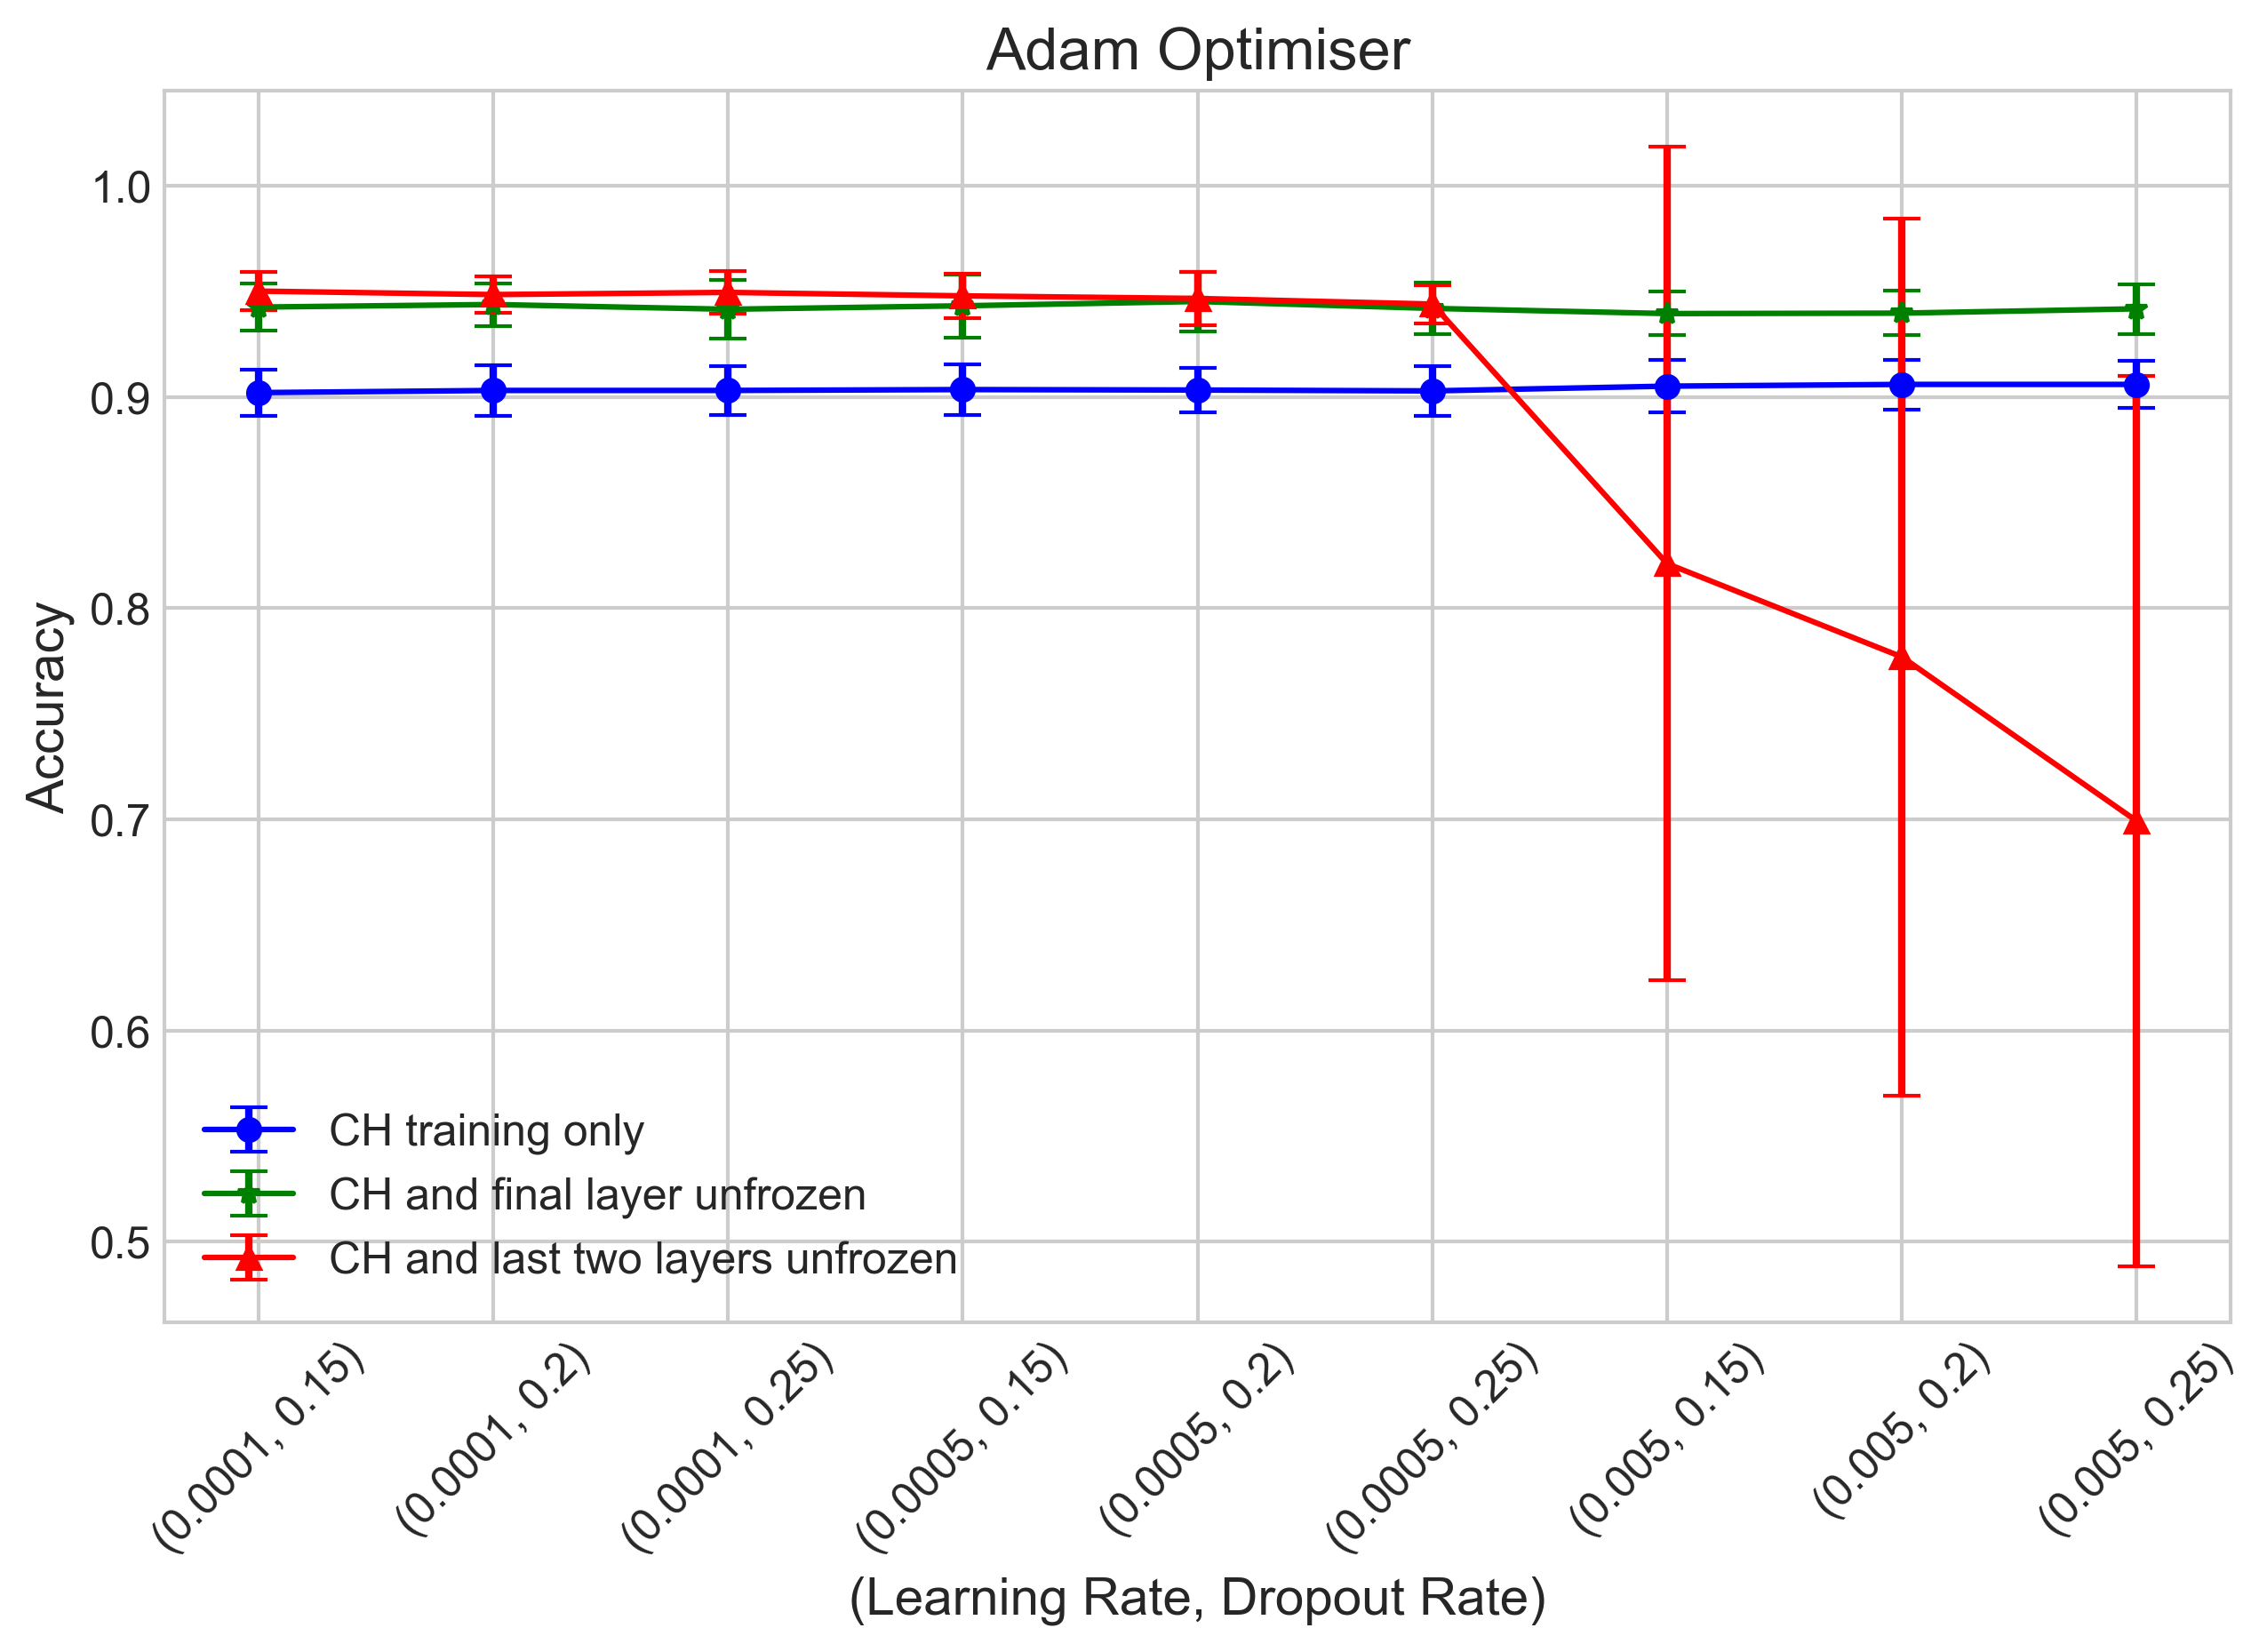
\includegraphics[width=\textwidth]{Adam_optimiser_accuracy.png}
		\end{subfigure}
        \hfill
		\begin{subfigure}[b]{\figwidthh}
			\caption{}
			\includegraphics[width=\textwidth]{Adam_optimiser_f1_score.png}
		\end{subfigure}
        \hfill
		\begin{subfigure}[b]{\figwidthh}
			\caption{}
			\includegraphics[width=\textwidth]{training_Adam_optimiser_TrainingTimeMin.png}
		\end{subfigure}
	\end{center}
	\caption{Results of fine-tuning using the Adam optimiser: (a) Accuracy of the validation data; (b) F-1 score on the validation data; (c) training time. 
	} 
	\label{fig:res_training_adam}
\end{figure}


\begin{figure}[p] 
	\begin{center}
		\begin{subfigure}[b]{\figwidthh}
			\caption{} 
			\includegraphics[width=\textwidth]{SGD_optimiser_accuracy.png}
		\end{subfigure}
        \hfill
		\begin{subfigure}[b]{\figwidthh}
			\caption{}
			\includegraphics[width=\textwidth]{SGD_optimiser_f1_score.png}
		\end{subfigure}
        \hfill
		\begin{subfigure}[b]{\figwidthh}
			\caption{}
			\includegraphics[width=\textwidth]{training_SGD_optimiser_TrainingTimeMin.png}
		\end{subfigure}
	\end{center}
	\caption{Results of fine-tuning using the SGD optimiser: (a) Accuracy of the validation data; (b) F-1 score on the validation data; (c) training time. 
	} 
	\label{fig:res_training_SGD}
\end{figure}

\newpage

%-------------------------------------------------------------------------------
% SECTION 2
%-------------------------------------------------------------------------------


\section{Prediction with fine-tuned models}

\begin{table}[h!]
	\caption{Prediction results on \inghamTwo using fine-tuned NN1 with the different optimisers and at different learning and drop out rates. }
	\centering
		\resizebox{\textwidth}{!}{%
		\begin{tabular}{@{}lcccccc@{}}
		\toprule
		&  \multicolumn{6}{c}{Accuracy (Learning rate, Drop out rate)} \\ \cmidrule(l){2-7} 
		Optimiser & (0.0001, 0.15) & (0.0001, 0.2) & (0.0001, 0.25) & (0.0005, 0.15) & (0.0005, 0.2) & (0.0005, 0.25) \\ \midrule
		Adam & $0.672 \pm 0.008$ & $0.672 \pm 0.009$ & $0.673 \pm 0.007$ & $0.683 \pm 0.009$ & $0.682 \pm 0.004$ & $0.686 \pm 0.009$ \\
		AdamW & $0.675 \pm 0.015$ & $0.682 \pm 0.011$ & $0.682 \pm 0.010$ & $0.695 \pm 0.012$ & $0.696 \pm 0.010$ & $0.693 \pm 0.008$ \\
		SGD & $0.521 \pm 0.034$ & $0.516 \pm 0.024$ & $0.519 \pm 0.024$ & $0.598 \pm 0.012$ & $0.596 \pm 0.012$ & $0.599 \pm 0.016$ \\
						\bottomrule
		\end{tabular}
		}

	\resizebox{\textwidth}{!}{%
    \begin{tabular}{@{}lcccccc@{}}
    \toprule
    &  \multicolumn{6}{c}{F1-score (Learning rate, Drop out rate)} \\ \cmidrule(l){2-7} 
    Optimiser & (0.0001, 0.15) & (0.0001, 0.2) & (0.0001, 0.25) & (0.0005, 0.15) & (0.0005, 0.2) & (0.0005, 0.25) \\ \midrule
	Adam & $0.612 \pm 0.013$ & $0.612 \pm 0.015$ & $0.611 \pm 0.015$ & $0.628 \pm 0.010$ & $0.629 \pm 0.008$ & $0.630 \pm 0.011$ \\
	AdamW & $0.616 \pm 0.019$ & $0.622 \pm 0.012$ & $0.621 \pm 0.012$ & $0.641 \pm 0.010$ & $0.640 \pm 0.009$ & $0.636 \pm 0.009$ \\
	SGD & $0.561 \pm 0.032$ & $0.566 \pm 0.018$ & $0.558 \pm 0.045$ & $0.553 \pm 0.015$ & $0.543 \pm 0.020$ & $0.558 \pm 0.019$ \\
			\bottomrule
    \end{tabular}
	}

	% \resizebox{\textwidth}{!}{%
    % \begin{tabular}{@{}lcccccc@{}}
    % \toprule
    % &  \multicolumn{6}{c}{Time (Sec) (Learning rate, Drop out rate)} \\ \cmidrule(l){2-7} 
	% 	\bottomrule
    % \end{tabular}
    % }
	
\end{table}
	

\begin{table}[h!]
	\caption{Prediction results on \inghamTwo using fine-tuned NN2 using the different optimisers and at different learning and drop out rates. }
	\centering
		\resizebox{\textwidth}{!}{%
		\begin{tabular}{@{}lcccccc@{}}
		\toprule
		&  \multicolumn{6}{c}{Accuracy (Learning rate, Drop out rate)} \\ \cmidrule(l){2-7} 
		Optimiser & (0.0001, 0.15) & (0.0001, 0.2) & (0.0001, 0.25) & (0.0005, 0.15) & (0.0005, 0.2) & (0.0005, 0.25) \\ \midrule
		Adam & $0.814 \pm 0.020$ & $0.818 \pm 0.010$ & $0.815 \pm 0.014$ & $0.818 \pm 0.016$ & $0.828 \pm 0.013$ & $0.824 \pm 0.014$ \\
		AdamW & $0.812 \pm 0.015$ & $0.820 \pm 0.013$ & $0.808 \pm 0.017$ & $0.828 \pm 0.010$ & $0.825 \pm 0.016$ & $0.818 \pm 0.014$ \\
		SGD & $0.596 \pm 0.028$ & $0.573 \pm 0.047$ & $0.593 \pm 0.031$ & $0.727 \pm 0.019$ & $0.722 \pm 0.026$ & $0.726 \pm 0.020$ \\
						\bottomrule
		\end{tabular}
		}

	\resizebox{\textwidth}{!}{%
    \begin{tabular}{@{}lcccccc@{}}
    \toprule
    &  \multicolumn{6}{c}{F1-score (Learning rate, Drop out rate)} \\ \cmidrule(l){2-7} 
    Optimiser & (0.0001, 0.15) & (0.0001, 0.2) & (0.0001, 0.25) & (0.0005, 0.15) & (0.0005, 0.2) & (0.0005, 0.25) \\ \midrule
	Adam & $0.756 \pm 0.019$ & $0.756 \pm 0.017$ & $0.756 \pm 0.019$ & $0.763 \pm 0.016$ & $0.775 \pm 0.021$ & $0.769 \pm 0.015$ \\
	AdamW & $0.762 \pm 0.014$ & $0.769 \pm 0.013$ & $0.761 \pm 0.011$ & $0.785 \pm 0.012$ & $0.781 \pm 0.020$ & $0.774 \pm 0.016$ \\
	SGD & $0.521 \pm 0.053$ & $0.547 \pm 0.049$ & $0.519 \pm 0.040$ & $0.686 \pm 0.020$ & $0.665 \pm 0.027$ & $0.677 \pm 0.013$ \\
			\bottomrule
    \end{tabular}
	}

	% \resizebox{\textwidth}{!}{%
    % \begin{tabular}{@{}lcccccc@{}}
    % \toprule
    % &  \multicolumn{6}{c}{Time (Min) (Learning rate, Drop out rate)} \\ \cmidrule(l){2-7} 
	% 	\bottomrule
    % \end{tabular}
    %}
		
\end{table}




\begin{figure}[p] 
	\begin{center}
		\begin{subfigure}[b]{\figwidthh}
			\caption{} 
			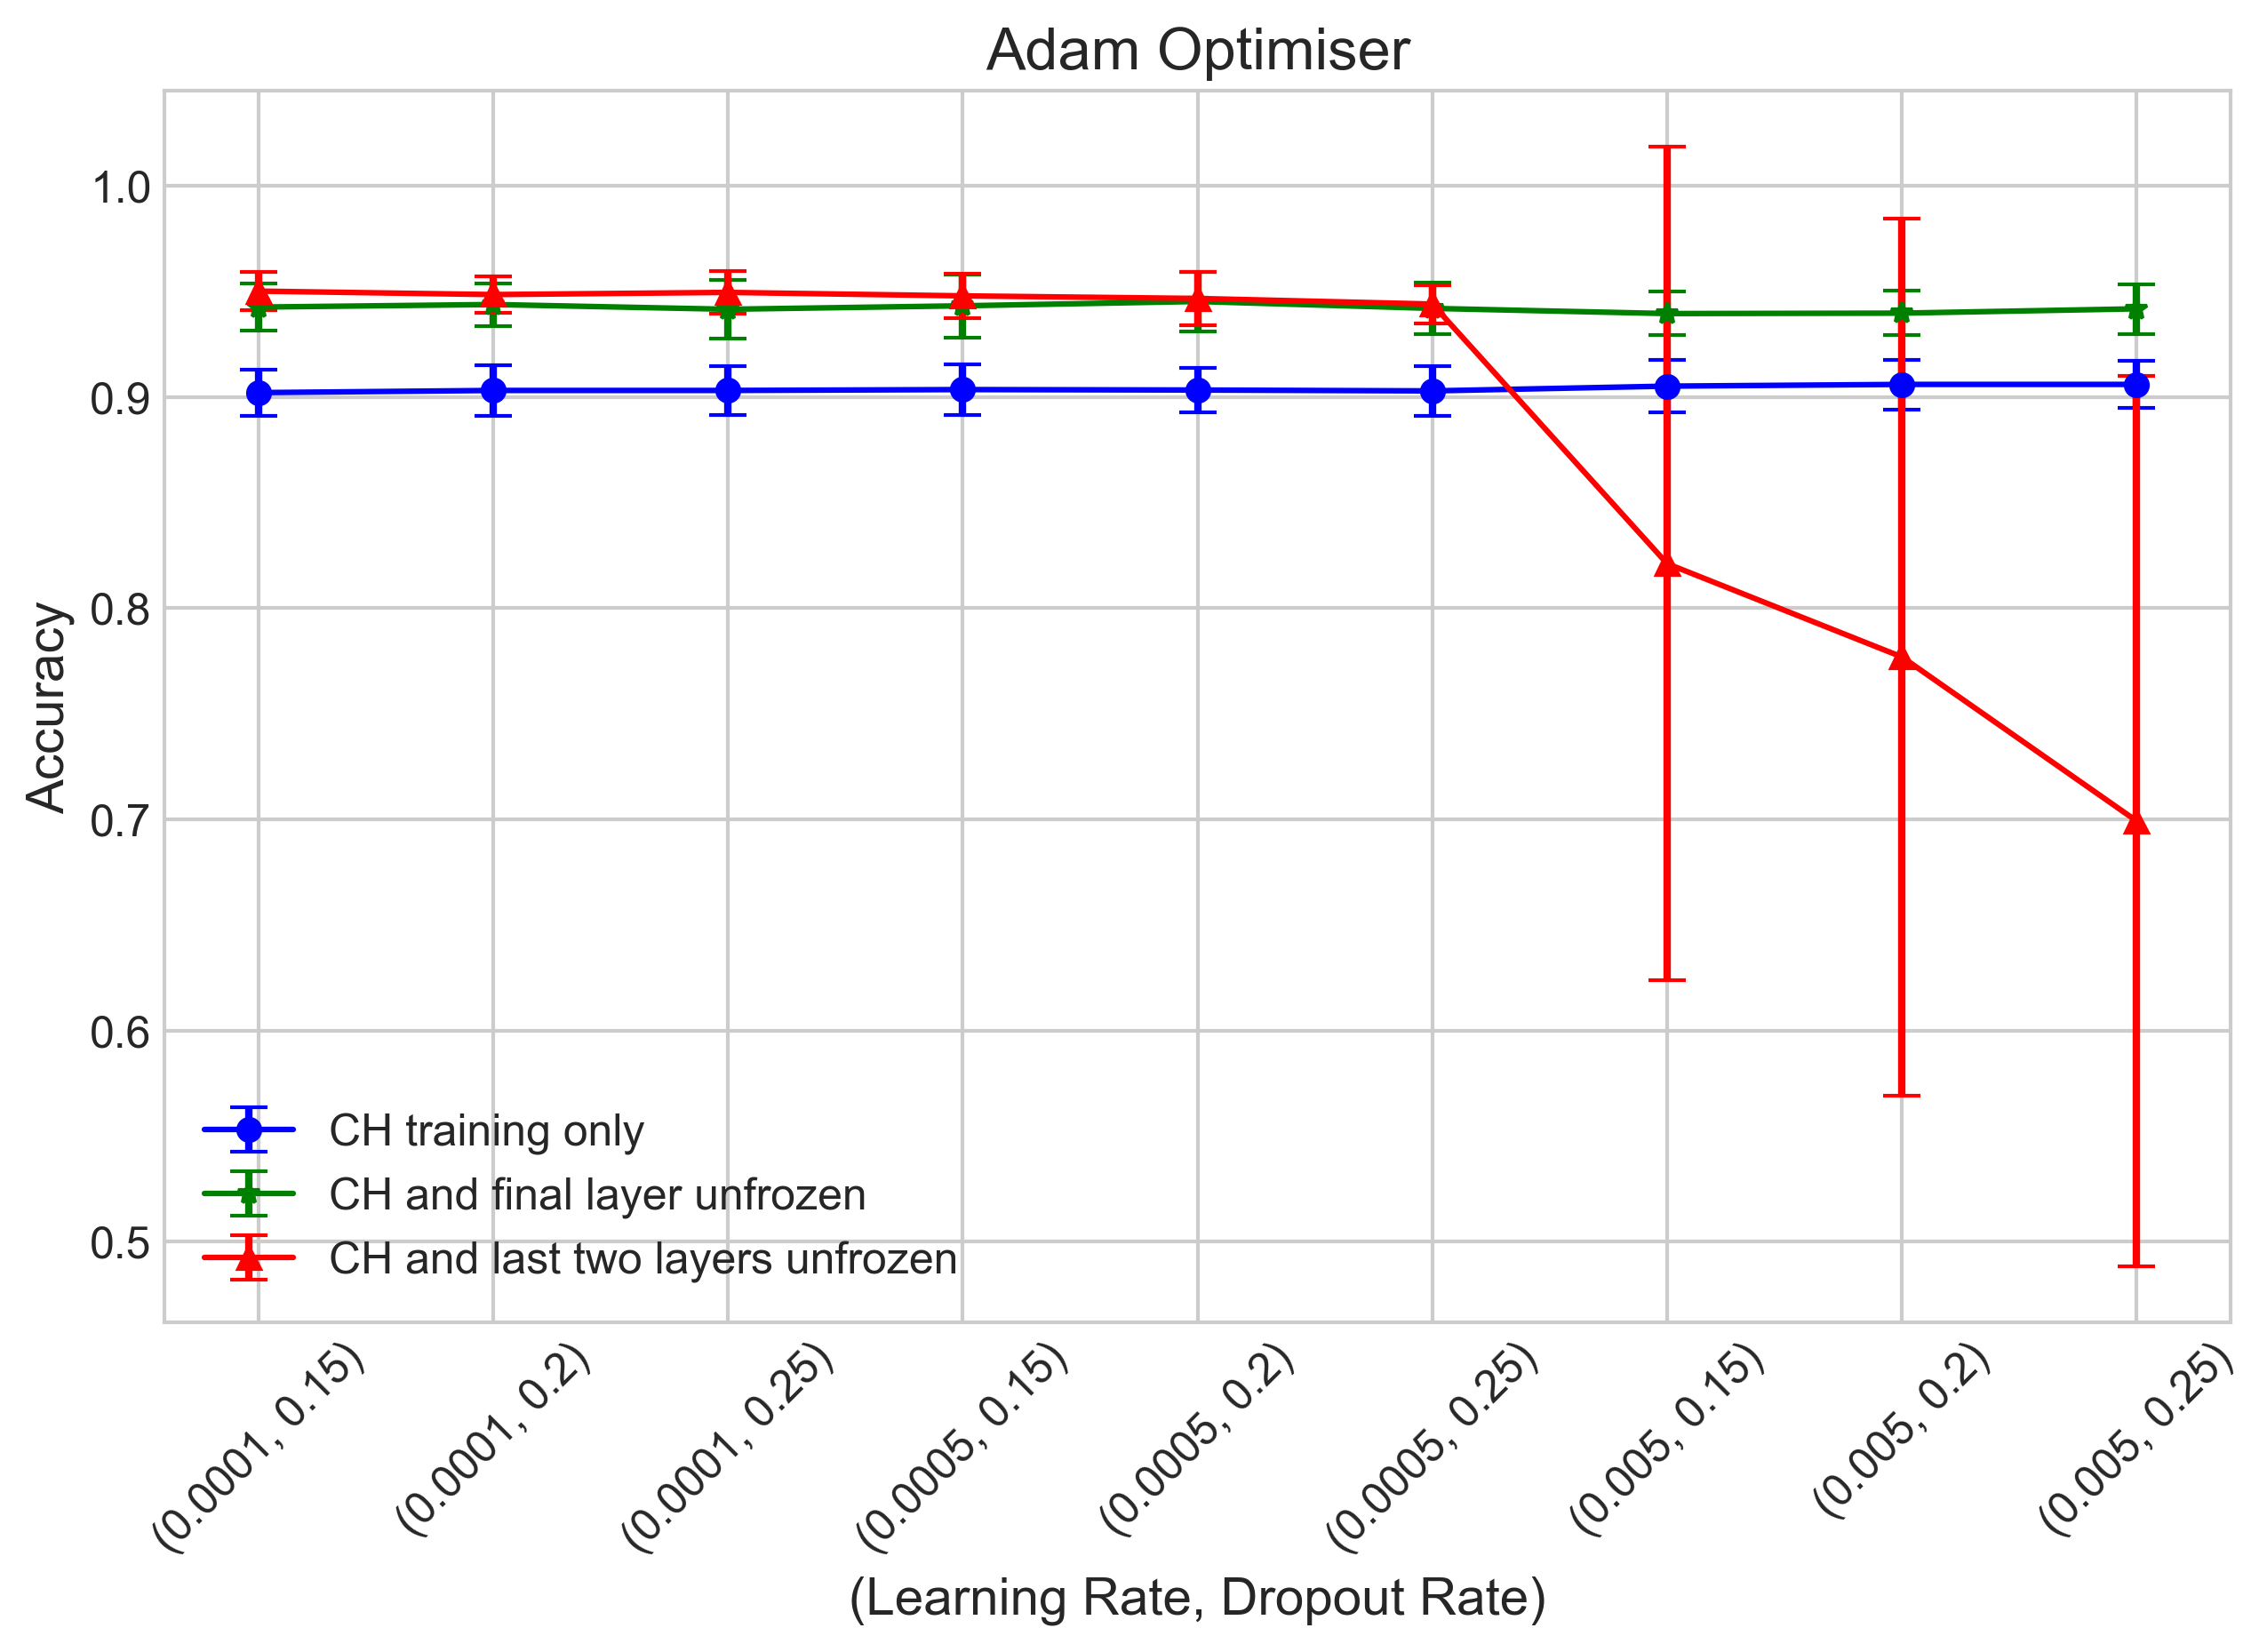
\includegraphics[width=\textwidth]{Adam_optimiser_accuracy.png}
		\end{subfigure}
        \hfill
		\begin{subfigure}[b]{\figwidthh}
			\caption{}
			\includegraphics[width=\textwidth]{Adam_optimiser_f1_score.png}
		\end{subfigure}
        \hfill
		\begin{subfigure}[b]{\figwidthh}
			\caption{}
			\includegraphics[width=\textwidth]{training_Adam_optimiser_TrainingTimeMin.png}
		\end{subfigure}
	\end{center}
	\caption{Results of prediction on In-house Two using models fine-tuned with the Adam optimiser: (a) Prediction accuracy; (b) F-1 score; (c) Prediction on CPU time.
	} 
	\label{fig:res_prdict_adam}
\end{figure}


\begin{figure}[p] 
	\begin{center}
		\begin{subfigure}[b]{\figwidthh}
			\caption{} 
			\includegraphics[width=\textwidth]{SGD_optimiser_accuracy.png}
		\end{subfigure}
        \hfill
		\begin{subfigure}[b]{\figwidthh}
			\caption{}
			\includegraphics[width=\textwidth]{SGD_optimiser_f1_score.png}
		\end{subfigure}
        \hfill
		\begin{subfigure}[b]{\figwidthh}
			\caption{}
			\includegraphics[width=\textwidth]{training_SGD_optimiser_TrainingTimeMin.png}
		\end{subfigure}
	\end{center}
	\caption{Results of prediction on In-house Two using models fine-tuned with the SGD optimiser: (a) Prediction accuracy; (b) F-1 score; (c) Prediction on CPU time.
	} 
	\label{fig:res_predict_SGD}
\end{figure}

\newpage


%-------------------------------------------------------------------------------
% SECTION 3
%-------------------------------------------------------------------------------

\section{Further fine-tuning on In-House One Data}

	
\begin{table}[h!]
	\caption{Accuracy, F1-score and training time on CPU of further fine-tuning (domain adaptation) on \inghamOne data with the different optimiser using NN2, 
	and at different learning and drop out rates.
	}
	\centering
		\resizebox{\textwidth}{!}{%
		\begin{tabular}{@{}lcccccc@{}}
		\toprule
		&  \multicolumn{6}{c}{Accuracy (Learning rate, Drop out rate)} \\ \cmidrule(l){2-7} 
	Optimiser & (0.0001, 0.15) & (0.0001, 0.2) & (0.0001, 0.25) & (0.0005, 0.15) & (0.0005, 0.2) & (0.0005, 0.25) \\ \midrule
	Adam & $0.936 \pm 0.008$ & $0.929 \pm 0.012$ & $0.928 \pm 0.011$ & $0.938 \pm 0.009$ & $0.943 \pm 0.011$ & $0.940 \pm 0.009$ \\
	AdamW & $0.923 \pm 0.011$ & $0.932 \pm 0.015$ & $0.922 \pm 0.013$ & $0.934 \pm 0.013$ & $0.941 \pm 0.013$ & $0.934 \pm 0.006$ \\
		\bottomrule
			\end{tabular}
		}
	
	\vspace{5mm}
		\resizebox{\textwidth}{!}{%
		\begin{tabular}{@{}lcccccc@{}}
		\toprule
		&  \multicolumn{6}{c}{F1 Score (Learning rate, Drop out rate)} \\ \cmidrule(l){2-7} 
	Optimiser & (0.0001, 0.15) & (0.0001, 0.2) & (0.0001, 0.25) & (0.0005, 0.15) & (0.0005, 0.2) & (0.0005, 0.25) \\ \midrule
	Adam & $0.930 \pm 0.009$ & $0.923 \pm 0.013$ & $0.922 \pm 0.011$ & $0.932 \pm 0.009$ & $0.937 \pm 0.013$ & $0.934 \pm 0.009$ \\
	AdamW & $0.916 \pm 0.011$ & $0.927 \pm 0.015$ & $0.916 \pm 0.014$ & $0.928 \pm 0.013$ & $0.936 \pm 0.014$ & $0.928 \pm 0.007$ \\
		\bottomrule
			\end{tabular}
		}
	\vspace{5mm}
	\resizebox{\textwidth}{!}{%
	\begin{tabular}{@{}lcccccc@{}}
	\toprule
	&  \multicolumn{6}{c}{Time (min) (Learning rate, Drop out rate)} \\ \cmidrule(l){2-7} 
Optimiser & (0.0001, 0.15) & (0.0001, 0.2) & (0.0001, 0.25) & (0.0005, 0.15) & (0.0005, 0.2) & (0.0005, 0.25) \\ \midrule
Adam & $198.092 \pm 59.439$ & $184.190 \pm 48.655$ & $185.488 \pm 45.923$ & $131.315 \pm 40.023$ & $127.185 \pm 63.776$ & $98.440 \pm 21.057$ \\
AdamW & $111.487 \pm 32.506$ & $104.337 \pm 24.244$ & $178.830 \pm 14.122$ & $166.618 \pm 32.676$ & $148.200 \pm 20.756$ & $93.328 \pm 21.506$ \\
	\bottomrule
		\end{tabular}
	}
	\end{table}
	
	
\begin{figure}[h!]
	\begin{center}
		\begin{subfigure}[b]{\figwidthhh}
			\caption{} 
			\includegraphics[width=\textwidth]{finetuning_Adam_optimiser_accuracy.png}
		\end{subfigure}
        \hfill
		\begin{subfigure}[b]{\figwidthhh}
			\caption{}
			\includegraphics[width=\textwidth]{finetuning_Adam_optimiser_f1_score.png}
		\end{subfigure}
        \hfill
		\begin{subfigure}[b]{\figwidthhh}
			\caption{}
			\includegraphics[width=\textwidth]{finetuning_Adam_optimiser_TrainingTimeMin.png}
		\end{subfigure}
	\end{center}                                                                
	\caption{Results of further fine-tuning on \inghamOne data with the Adam optimiser: (a) Prediction accuracy; (b) F-1 score; (c) Training time on CPU (min).
	} 
\end{figure}


\newpage
%-------------------------------------------------------------------------------
% SECTION 4
%-------------------------------------------------------------------------------


\section{Prediction with domain adapted models}

\begin{table}[h!]
	\caption{Accuracy, F1-score and training time on CPU of further fine-tuning (domain adaptation) on \inghamOne data with the different optimiser using NN2, 
	and at different learning and drop out rates.
	}
	\centering
		\resizebox{\textwidth}{!}{%
		\begin{tabular}{@{}lcccccc@{}}
		\toprule
		&  \multicolumn{6}{c}{Accuracy (Learning rate, Drop out rate)} \\ \cmidrule(l){2-7} 
		Optimiser & (0.0001, 0.15) & (0.0001, 0.2) & (0.0001, 0.25) & (0.0005, 0.15) & (0.0005, 0.2) & (0.0005, 0.25) \\ \midrule
		Adam & $0.933 \pm 0.004$ & $0.931 \pm 0.005$ & $0.930 \pm 0.004$ & $0.933 \pm 0.005$ & $0.935 \pm 0.004$ & $0.932 \pm 0.006$ \\
		AdamW & $0.925 \pm 0.006$ & $0.923 \pm 0.005$ & $0.923 \pm 0.007$ & $0.930 \pm 0.003$ & $0.931 \pm 0.005$ & $0.928 \pm 0.005$ \\
		\bottomrule
		\end{tabular}
		} 

	\vspace{5mm}
		\resizebox{\textwidth}{!}{%
		\begin{tabular}{@{}lcccccc@{}}
		\toprule
		&  \multicolumn{6}{c}{F1 Score (Learning rate, Drop out rate)} \\ \cmidrule(l){2-7} 
	Optimiser & (0.0001, 0.15) & (0.0001, 0.2) & (0.0001, 0.25) & (0.0005, 0.15) & (0.0005, 0.2) & (0.0005, 0.25) \\ \midrule
	Adam & $0.922 \pm 0.005$ & $0.920 \pm 0.006$ & $0.919 \pm 0.005$ & $0.922 \pm 0.005$ & $0.924 \pm 0.004$ & $0.920 \pm 0.006$ \\
	AdamW & $0.913 \pm 0.007$ & $0.911 \pm 0.005$ & $0.911 \pm 0.007$ & $0.918 \pm 0.004$ & $0.919 \pm 0.006$ & $0.916 \pm 0.006$ \\
			\bottomrule
		\end{tabular}
		}
\end{table}


\begin{figure}[h!]
	\begin{center}
		\begin{subfigure}[b]{\figwidthhh}
			\caption{} 
			\includegraphics[width=\textwidth]{finetune_prediction_Adam_optimiser_accuracy.png}
		\end{subfigure}
        \hfill
		\begin{subfigure}[b]{\figwidthhh}
			\caption{}
			\includegraphics[width=\textwidth]{finetune_prediction_Adam_optimiser_f1_score.png}
		\end{subfigure}
        \hfill
		\begin{subfigure}[b]{\figwidthhh}
			\caption{}
			\includegraphics[width=\textwidth]{finetune_prediction_Adam_optimiser_PredictTimeSeconds.png}
		\end{subfigure}
	\end{center}
	\caption{Results of prediction on \inghamTwo data with the domain adapted models optimised with Adam optimiser: (a) Prediction accuracy; (b) F-1 score; (c) Time taken on CPU (s)
	} 
\end{figure}

\end{document}